\chapter{DESIGN METHODOLOGY OF BULK EMAIL MANAGEMENT SYSTEM}
\label{design_meth}

\section{UML Diagrams}
The Unified Modelling Language (UML) is a standard language for writing software blueprints. UML can be used for:

\begin{itemize}
  \item \textbf{Specifying}: It is a blueprint created by an architect prior to the construction.
  \item \textbf{Visualizing} : Visualizing is concerned with deep analysis of system to be constructed.
  \item \textbf{Constructing} : Modelling also provide us mechanism which are essential while
constructing a system.
 \item \textbf{Documenting} : Finally, modelling justifies its importance by applying all its credentials
to be bounded in a piece of paper referred as document. 

\end{itemize}

The UML is a language which provides vocabulary and the rules for combining words in that vocabulary for the purpose of communication. A modelling language is a language whose
vocabulary and the rules focus on the conceptual and physical representation of a system. Modelling yields an understanding of a system.

Three types of diagrams are shown to propose the design and depict the methodology that is implemented by using the appropriate tools.

\subsection{Use Case Diagram}

\begin{figure}[H]
            \centering
            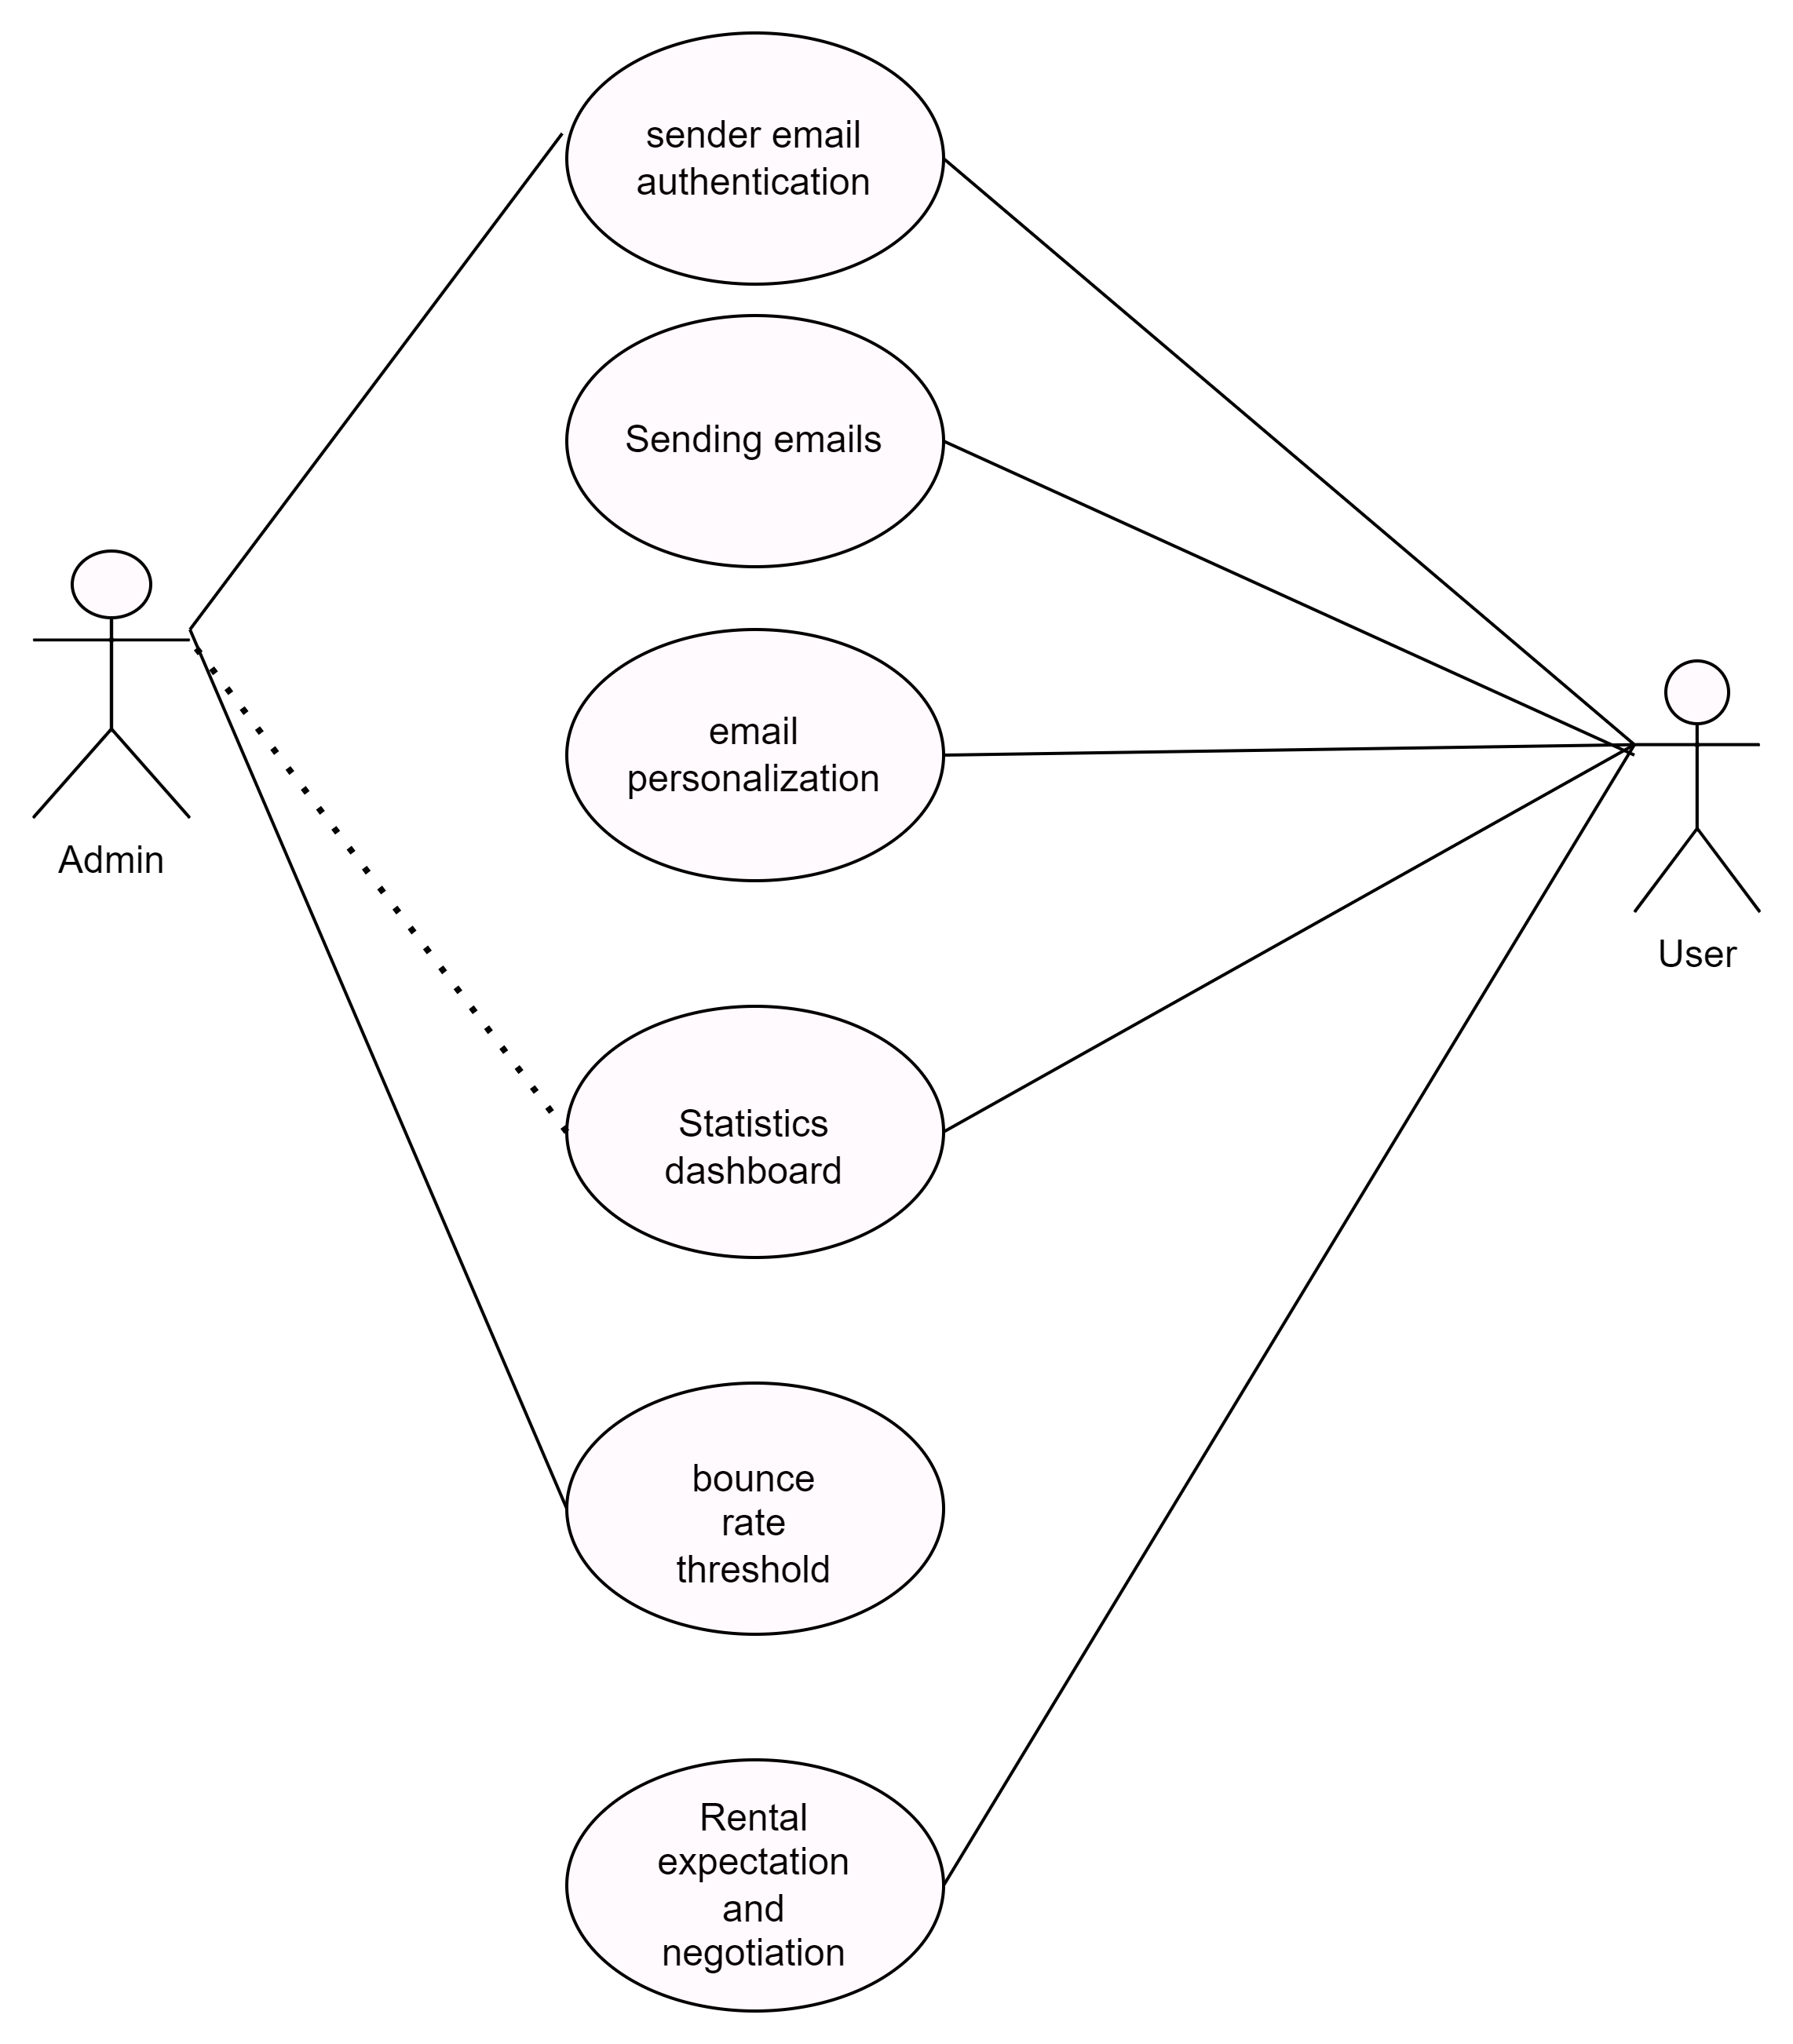
\includegraphics[width=160mm, height=100mm]{figures/use_case.png}
            \caption{Use case Diagram}
            \label{fig:use-case-diagram}
\end{figure}

Use case diagrams are used to gather the requirements of a system including internal and external influences. These requirements are mostly design requirements. So, when a system
is analyzed together its functionalities use cases are prepared and actors are identified. 

In Figure \ref{fig:use-case-diagram}, the user gives in Input Program to the compiler and is able to view the outcomes of Syntax, Lexical analysis phases of the compilation process (compilation errors if any in the source code).

 

\section{Data Flow Diagram}

A data-flow diagram is a way of representing a flow of data through a process or a system (usually an information system). The DFD also provides information about the outputs and inputs of each entity and the process itself. A data-flow diagram has no control flow, there are no decision rules and no loops. Specific operations based on the data can be represented by
a flowchart. 

For each data flow, at least one of the endpoints (source and / or destination) must exist in a process. The refined representation of a process can be done in another data-flow diagram, which subdivides this process into sub-processes.



\begin{figure}[H]
            \centering
            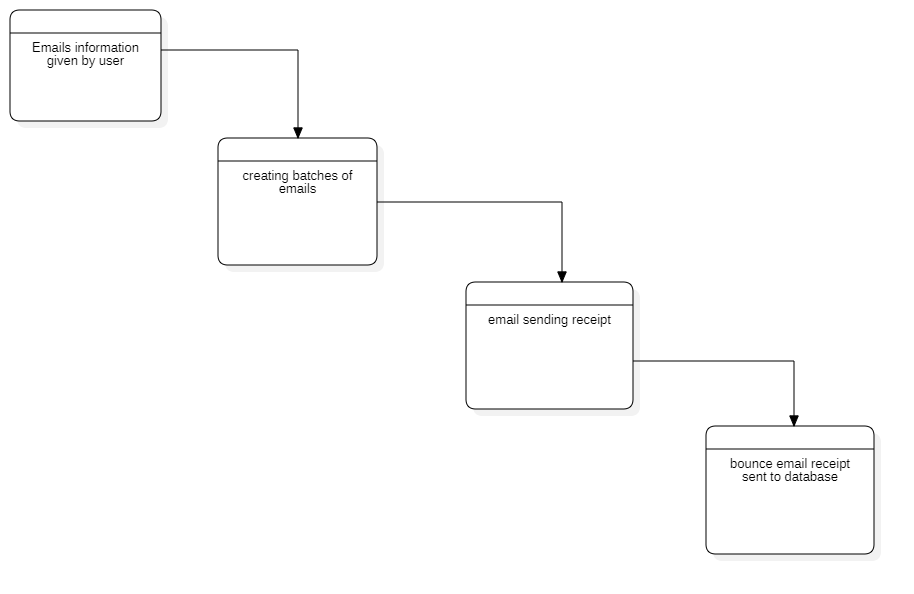
\includegraphics[width=160mm]{figures/data_flow_diagram.png}
            \caption{Data Flow Diagram of bulk email management system}
	    \label{fig:data-flow-diagram}
\end{figure}


The data flow diagram displayed in Figure \ref{fig:data-flow-diagram} shows how the data that is entered by the user is processed till the sending of emails and further finding the bounce emails data and how they are stored finally in a database.

\section{Architecture diagram}

Architecture diagram shows how various components that exists in a network work together and are integrated with other services. User interaction to output the various methods and services used and their correlation is depicted in this diagram.

The components used can be instances of a component and the sequence in which they need to be connected to successfully achieve the desired output is shown here.

\begin{figure}[H]
            \centering
            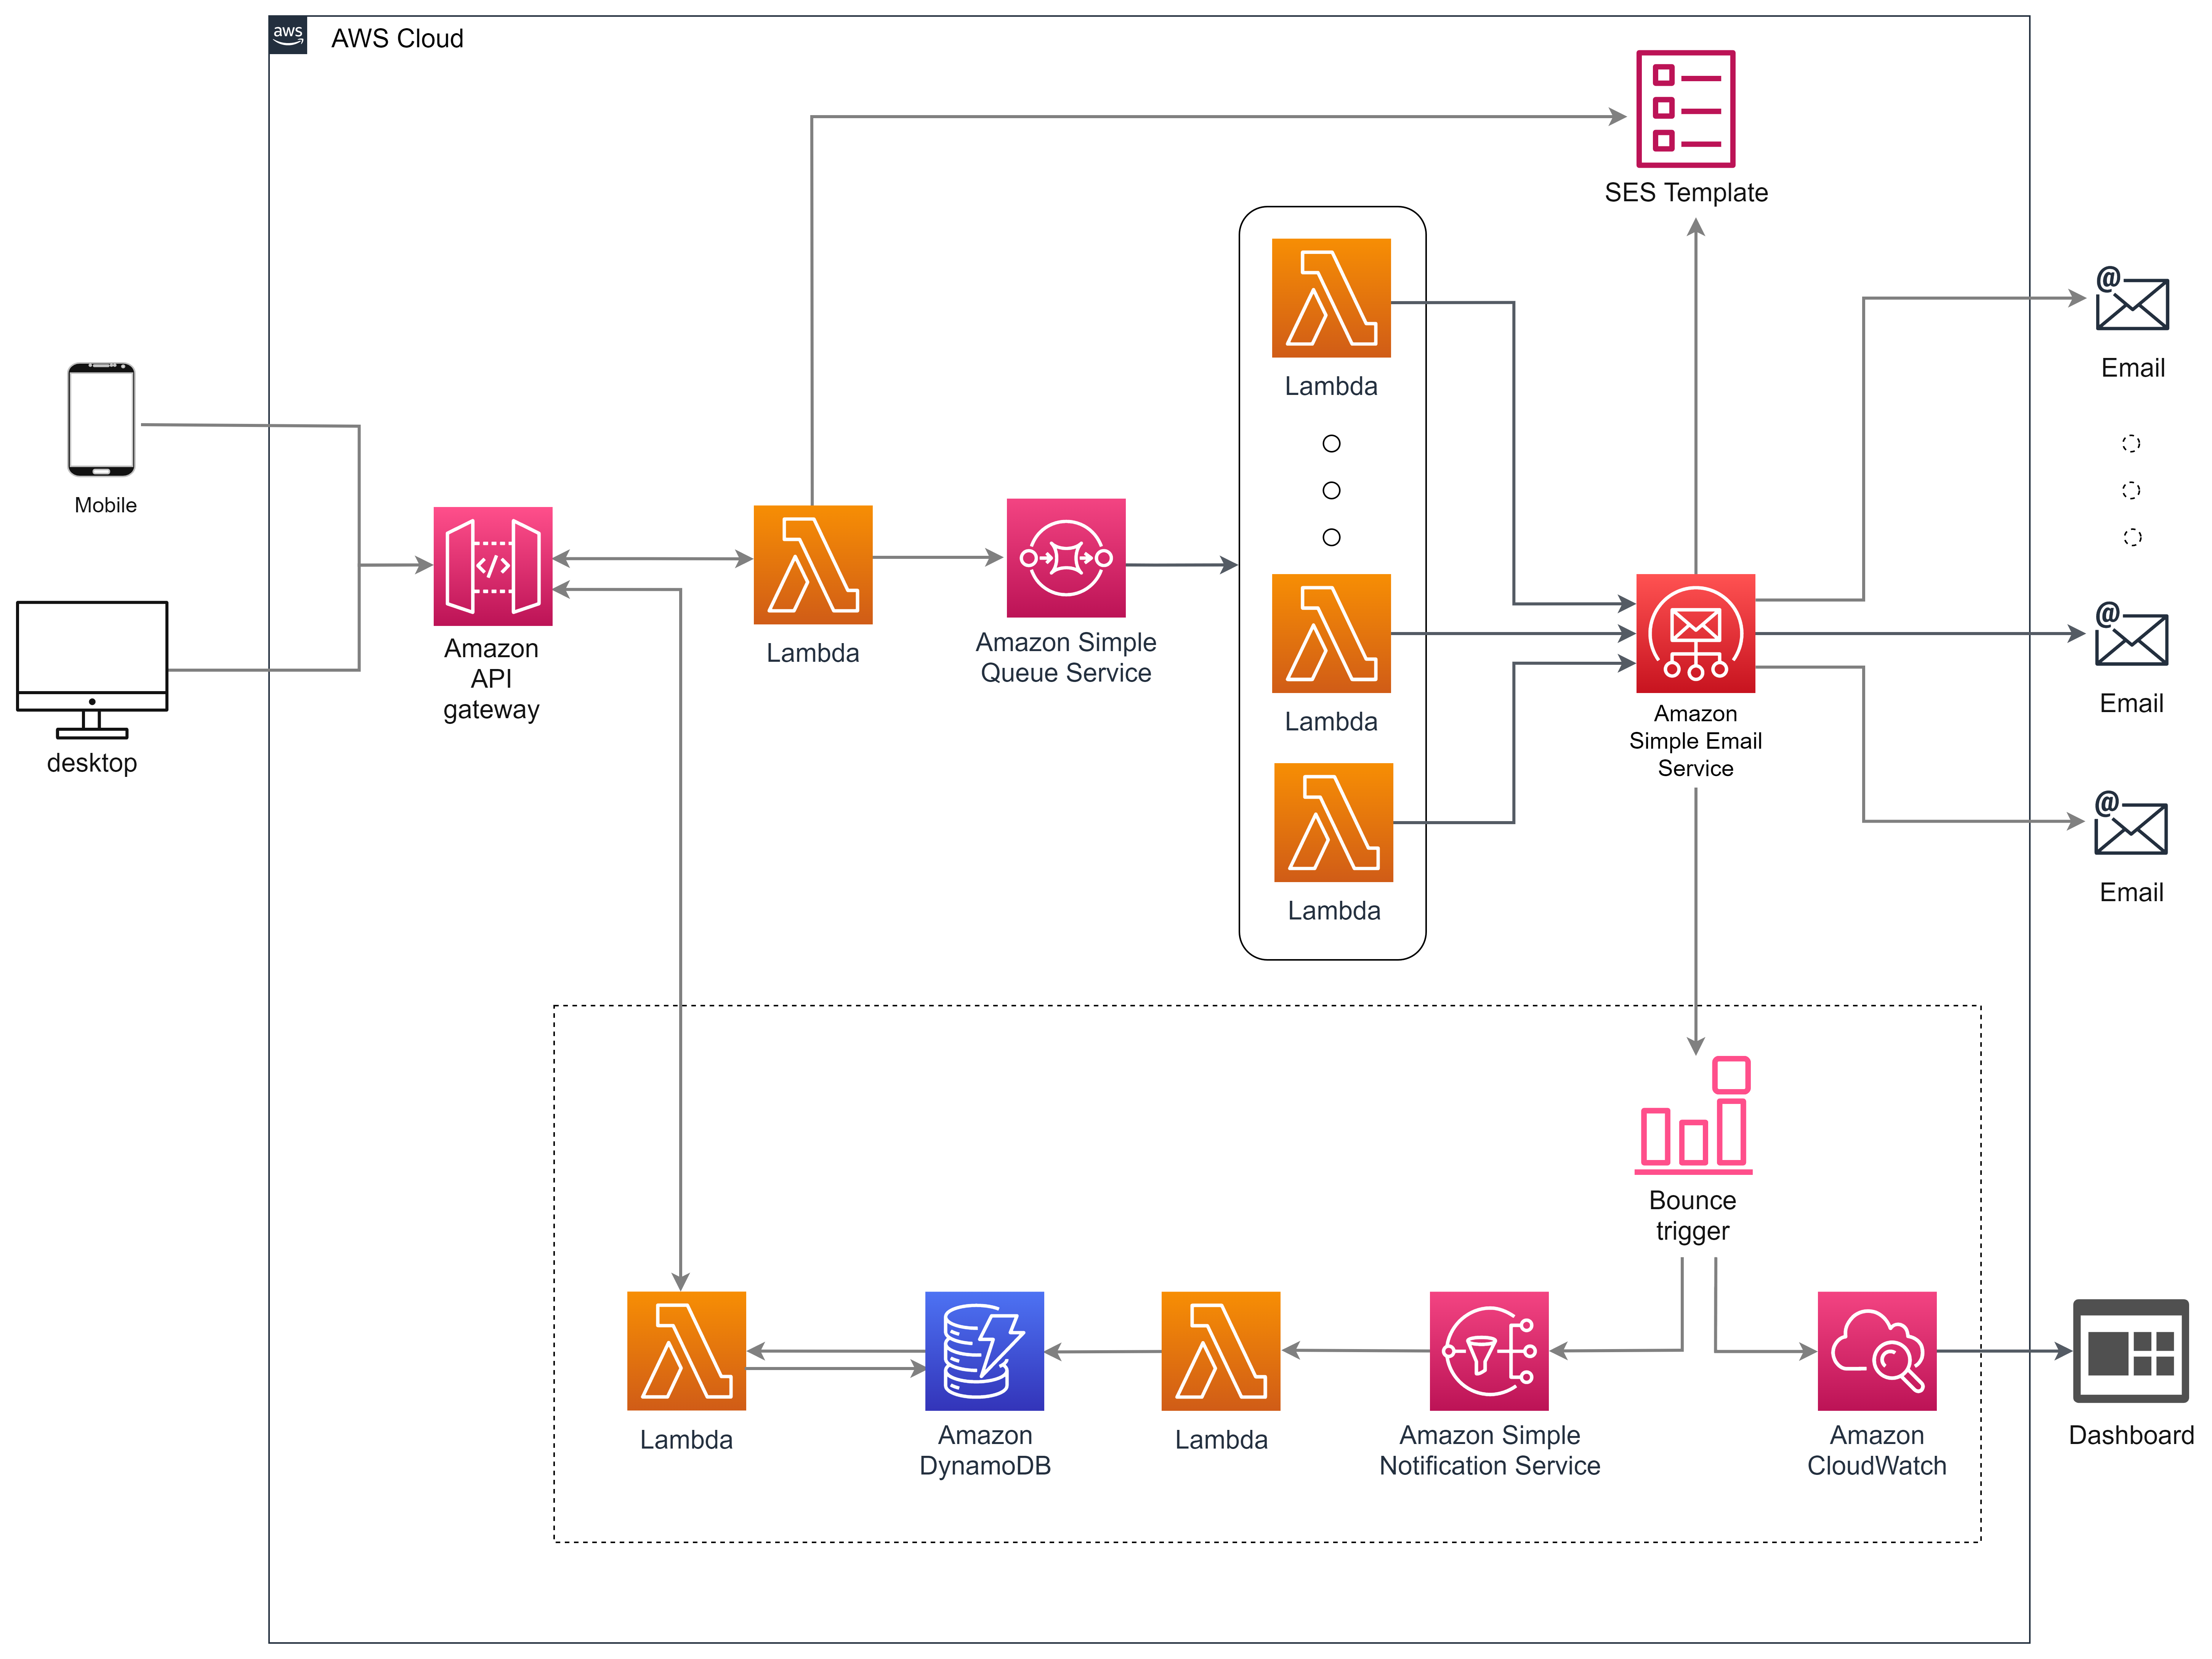
\includegraphics[width=160mm]{figures/architect.png}
            \caption{AWS architecture of bulk email management system}
	    \label{fig:architect}
\end{figure}


The data flow diagram displayed in Figure \ref{fig:architect} shows how the data that is entered by the user is processed till the sending of emails and further finding the bounce emails data and how they are stored finally in a database.

The architecture is based a few constraints from the SES service and other bottlenecks that affect the sending of emails. The SES through which the emails are initially sent through sandbox to test and later needs to be upgraded by the AWS authority to permit the user to request increase in the number of emails to be sent. For the purpose of this architecture 50,000 emails have been requested which was granted by the authority.
\begin{itemize}
	\item 14 emails/second
	\item 50,000 emails per day
	\item request data 5kb
\end{itemize}

